\documentclass{article}
\usepackage{fullpage}
\usepackage{amsmath, amssymb}
\usepackage[hidelinks]{hyperref}
\usepackage[utf8]{inputenc}
\usepackage{natbib}
\usepackage{graphicx}
\usepackage{enumitem}
\usepackage{listings}
\bibliographystyle{plainnat}
% \usepackage[T1]{fontenc}


\newcommand{\R}{\mathbb{R}}
\newcommand{\Q}{\mathbb{Q}}
\newcommand{\Z}{\mathbb{Z}}
\newcommand{\N}{\mathbb{N}}
\newcommand{\C}{\mathbb{C}}

\renewcommand{\P}{\mathbb{P}}
\newcommand{\E}{\mathbb{E}}
\newcommand{\var}{\mathop{\mbox{Var}}}
\newcommand{\cov}{\mathop{\mbox{cov}}}
%\newcommand{\det}{\mathop{\mbox{det}}}
\newcommand{\supp}{\mathop{\mbox{supp}}}
\newcommand{\sgn}{\mathop{\mbox{sgn}}}
\newcommand{\EE}[1]{\E\!\left[#1\right]}
\newcommand{\PP}[1]{\P\!\left\{#1\right\}}
\newcommand{\PPP}[2]{\P_{#1}\!\left\{#2\right\}}
\newcommand{\EEE}[2]{\E_{#1}\!\left[#2\right]}
\newcommand{\EEsup}[2]{\E^{#1}\!\left[#2\right]}

\newcommand{\bone}{\mathbf{1}}

% These macros are borrowed from TAOCPMAC.tex
\newcommand{\slug}{\hbox{\kern1.5pt\vrule width2.5pt height6pt depth1.5pt\kern1.5pt}}
\def\xskip{\hskip 7pt plus 3pt minus 4pt}
\newdimen\algindent
\newif\ifitempar \itempartrue % normally true unless briefly set false
\def\algindentset#1{\setbox0\hbox{{\bf #1.\kern.25em}}\algindent=\wd0\relax}
\def\algbegin #1 #2{\algindentset{#21}\alg #1 #2} % when steps all have 1 digit
\def\aalgbegin #1 #2{\algindentset{#211}\alg #1 #2} % when 10 or more steps
\def\alg#1(#2). {\medbreak % Usage: \algbegin Algorithm A (algname). This...
  \noindent{\bf#1}({\it#2\/}).\xskip\ignorespaces}
\def\kalgstep#1.{\ifitempar\smallskip\noindent\else\itempartrue
   \hskip-\parindent\fi
   \hbox to\algindent{\bf\hfil #1.\kern.25em}%
   \hangindent=\algindent\hangafter=1\ignorespaces}

\newcommand{\algstep}[3]{\kalgstep #1 [#2] #3 }
\newenvironment{taocpalg}[3]{%
\vspace{1em}%
\algbegin Algorithm #1. ({#2}). #3 }
{\vspace{1em}}

\newcommand{\randomuniform}[0]{\mathcal{R}_U}
\newcommand{\randomdiscrete}[0]{\mathcal{R}_D}
\newcommand{\algref}[1]{#1}

% \newcommand{\tablenotation}[1]{\mathcal{#1}}
% \newcommand{\tableaddrow}[0]{\mbox{add}}

\newcommand{\simupop}{\texttt{simuPOP}}
\newcommand{\fwdpp}{\texttt{fwdpp}}
\newcommand{\fwdpy}{\texttt{fwdpy11}}
\newcommand{\msprime}{\texttt{msprime}}
\newcommand{\ftprime}{\texttt{ftprime}}
\newcommand{\nodes}{\texttt{nodes}}
\newcommand{\edgesets}{\texttt{edgesets}}
\newcommand{\sites}{\texttt{sites}}
\newcommand{\mutations}{\texttt{mutations}}
\newcommand{\setdiff}{\smallsetminus}
\newcommand{\Nt}{\mathcal{N}}  % node table
\newcommand{\Et}{\mathcal{E}}  % edge table
\newcommand{\St}{\mathcal{S}}  % site table
\newcommand{\Mt}{\mathcal{M}}  % mutation table
\newcommand{\Al}{\mathcal{A}}  % list of ancestors
\newcommand{\taddnode}[1]{\mbox{addnode}(#1)}
\newcommand{\taddedge}[1]{\mbox{addedge}(#1)}
\newcommand{\tsimplify}[1]{\mbox{simplify}(#1)}
\DeclareMathOperator{\len}{length}
\DeclareMathOperator{\add}{add} % for adding to tables
\newcommand{\lleft}{\mathrm{left}}  % left label
\newcommand{\lright}{\mathrm{right}}
\newcommand{\lid}{\mathrm{id}}

\usepackage{color}
\newcommand{\krt}[1]{{\em \color{green} #1}}
\newcommand{\plr}[1]{{\em \color{blue} #1}}
\newcommand{\jk}[1]{{\em \color{red} #1}}
\newcommand{\jda}[1]{{\em \color{cyan} #1}}

\begin{document}

\title{Efficient pedigree recording for fast population genetics simulation}
\author{Jerome Kelleher,
        Kevin R. Thornton,
        Jaime Ashander, and
        Peter L. Ralph}
\maketitle



\begin{abstract}
    In this paper we describe how to
    efficiently record the entire genetic history of a population
    during a forwards-time, individual-based population genetics simulation.
    This allows us to dramatically reduce the computational burden of tracking individual genomes
    by simulating only those loci that may affect reproduction (those having non-neutral variants),
    and recording history in the \emph{tree sequence} format introduced in the software package \msprime,
    on which neutral mutations can be quickly placed afterwards.
    We implement the method in two popular forwards-time simulation frameworks,
    and show that not only does this speed up large simulations by one or two orders of magnitude,
    but saves substantially more information from the simulation
    (all marginal genealogies).
    % This has the promise of making large-scale, whole-genome simulations with realistic geography and selection finally possible.
\end{abstract}

% NOTE: I tend to use semantic linebreaks.
% Please excuse the ragged right margins in the source.


%%%%%%%%%%%%%%%%%%%%%%
\section*{Introduction}

Since the 1980's, coalescent theory has enabled computer simulation of the results of population genetics models
identical to that which would be produced by large, randomly mating populations over long periods of time
without actually requiring simulation of so many generations or meioses.
Coalescent theory thus had three transformative effects on population genetics:
first, giving researchers better conceptual tools to describe \emph{gene trees} and thus bringing within-population trees into better focus;
second, producing analytical methods to estimate parameters of interest from genetic data (e.g., $\theta = 4N_e \mu$);
and finally, providing a computationally feasible method to produce computer simulations of population genetics processes.
However, these powerful advances came with substantial caveats:
the backwards-in-time processes that are described by coalescent theory
are only \emph{Markovian}, and thus feasible to work with,
thanks to the important assumptions of
(a) random mating,
(b) neutrality,
and (c) small sample size relative to the population size.
The first two assumptions can be side-stepped to a limited extent,
but it remains a challenge to map results of coalescent models
onto species that are distributed across continuous geographical space
and/or have large numbers of loci under various sorts of selection.
Furthermore, the relationship between the life history of a species --
fecundity and mortality schedules, density-dependent effects on fitness, and demographic fluctuations --
are all absorbed into a single compound parameter, the coalescence rate.
The third assumption is no longer safe, either --
for example, a recent study~\citep{martin2017human}
simulated 600,000 samples of human chromosome 20 to examine biases in GWAS.
Several studies have now shown that in samples of size approaching that of the population,
genealogical properties may be distorted relative to the coalescent expectation
\citep{wakeley2003gene,maruvka2011recovering,bhaskar2014distortion}.
These considerations, and increasing computational power, have led to a resurgence of
interest in large forwards-time, individual-based simulations.
For instance, \citet{harris2016genetic} used SLiM \citep{slim} to simulate ten thousand human exomes
to assess the impact of genetic load and Neanderthal introgression on human genetic diversity.
\cite{Sanjak2017-ko} used
fwdpp \citep{fwdpp} to simulate a series of models of quantitative traits under mutation-selection balance with
population sizes of $2 \times 10^4$ diploids in stable populations and populations growing up to $\sim 5
\times 10^5$ individuals, using the output to explore the relationship between the genotype/phenotype model and GWAS
outcomes.

Modern computing power easily allows simulations of birth, death and reproduction
in a population having even hundreds of millions of individuals.
However, if our interest lies in the resulting genetic patterns of variation
-- and often, the point of such simulations is to compare to real data --
then such simulations must somehow produce at the end data for each individual on a genomic scale.
As samples of most species' genomes harbor tens or hundreds of millions of variant sites,
naively carrying full genotypes for even modest numbers of individuals through a simulation
becomes quickly prohibitive.
To make matters worse,
a population of size $N$ must be simulated across many multiples of $N$ generations
to produce stable genetic patterns.
Because of this computational burden of neutral mutations, even the fastest simulation frameworks such as SLiM,
SLiM2~\citep{haller2017flexible} and fwdpp~\citep{fwdpp}
can ``only'' simulate tens of megabases of sequence in tens of thousands of individuals
for tens of thousands of generations, and there are still near-order-of-magnitude performance differences between these
implementations~\citep{haller2017flexible}.
In practice, current state-of-the-art simulation software may take on the order of
weeks to simulate models of large genomic regions without selection~\citep{fwdpp,Hernandez2015-wf},
and existing simulation engines differ in how efficiently they
calculate fitnesses in models with selection~\citep{fwdpp}.
These population and region sizes are still substantially short of whole genomes
(hundreds to thousands of megabases)
for many biological population sizes of interest.

However, it is thought that most genetic variation is selectively neutral (or nearly so).
By definition, the neutral alleles carried by individuals in a population
do not affect the population process.
For this reason, if one records the entire genealogical history of a population over the course of a simulation,
simply laying down neutral mutations on top of that history afterwards
is equivalent to having generated them during the simulation.
Precisely, we would need to know the genealogical tree relating all sampled individuals
at each position along the genome.
In this paper, we describe how algorithmic tools and data structures developed for the
coalescent simulator \msprime{}
can be used to efficiently record, and later process, this history.
In so doing we record the \emph{population pedigree} --
the complete history of parent-offspring relationships of an entire population
going back to a remote time including the genetic outcomes of each ancestral
meiosis.
This embellished pedigree contains all the information necessary
to construct the genealogical tree that relates each individual to each other
at each position on the genome, i.e., the \emph{tree sequence}~\citep{kelleher2016efficient}.
Combined with ancestral genotypes and the origins of new mutations,
it also completely specifies the genomic sequence of any individual in the population at any time.
This is much more than we need to know, however,
so we discard all information irrelevant to the genetic history
of the extant population. We show that we need only $O(N \log N)$
space to store the resulting tree sequence for a single crossover per
generation under the Wright-Fisher model.

In this paper we discuss storage methods for genealogies (and hence, genome sequence),
an algorithm for simplifying these,
and their use in forwards-time simulation.
Although we were motivated by a need for more efficient genomic simulations,
these tools may prove more widely useful.


%%%%%%%%%%%%%%%%%%%%%
\section*{Results}


We begin by benchmarking the performance improvement achieved by connecting
two previously published forwards-time simulation libraries,
\simupop{} \citep{peng2005simupop} and \fwdpp{} \citep{fwdpp}
to the tools we describe here, as implemented in \msprime{}.
Then, we describe the conceptual and algorithmic foundations for the method:
(a) a format, implemented in the \msprime{} Python API,
for recording tree sequences in several \emph{tables};
(b) an algorithm to record tree sequence information into these tables on the fly
    from a forwards-time simulation;
and (c) an algorithm to \emph{simplify} a tree sequence, i.e., remove redundant information.
Finally, we analyze the run time and space complexity of our general-purpose method.


%%%%%%
\subsection*{Simulation benchmarks}

To measure the performance gains from recording the pedigree we ran simulations both with and without recording.
All simulations implemented a discrete-time Wright-Fisher population of diploid
population size $N$, simulated for $10N$ generations.
The simulations without pedigree recording introduced neutral mutations at a rate
equal to the recombination rate,
so $\mu = r$, where $\mu$ and $r$ are the expected number of mutations per gamete and recombination breakpoints per
diploid,
respectively, each generation. 
% Both mutations and recombinations occur as Poisson processes with respective means $\mu$ and $r$,
% and we used the infinitely-many sites mutation model \citep{Kimura1969-uc}.
We ran simulations with different values of $N$ and varied the size of the region according to the scaled recombination
parameter $\rho = 4Nr$.  When simulating neutral mutations, we kept the scaled mutation parameter, $\theta = 4N\mu$
equal to $\rho$.

Deleterious mutations were introduced at rate $\rho/100$ per generation, drawing scaled selection
coefficients ($2Ns$)
from a Gamma distribution with a mean of -5 and a shape parameter of 1.  This distribution of fitness effects results in
thousands of weakly-deleterious mutations segregating in the population, many of which drift to intermediate
frequencies.  The case of many mutations with selection is a non-trivial violation of exchangeability assumptions of the
coalescent \citep{Neuhauser1997-nn}.  Therefore, these selected mutations must be explicitly tracked in our forward simulation
and the time savings due to pedigree recording come from not having to record \textit{neutral} mutations.

To demonstrate the method's flexibility and to test it in different contexts,
we implemented these simulations separately using two different simulation engines:
\begin{enumerate}

    \item
        In C++, using \fwdpp{} library functions and interface code (details below),
        using a continuum-sites model for both mutation and recombination. Simulations were run using \fwdpy{}, a Python
        package based on \fwdpp.
        % $\mu$ and $r$ were the means of Poisson processes,
        % and mutations used the infinite-sites model \citep{Kimura1969-uc}.
        % We varied $N \in (1000, 10000, 50000)$, $\rho \in (10^3, 10^4, 10^5)$.

    \item
        In Python, using the \simupop{} library interfacing with a custom Python library (\ftprime{}),
        using a discrete but large number of sites.
        % $\mu$ and $r$ define per-base-pair mutation rate and we
        % defined the length of the simulated sequence, in base pairs, as $L = \tfrac{\rho}{4N \mu}$.
        % We varied $N \in (1000, 10000)$, $\rho \in (10^3, 10^4)$.

\end{enumerate}

We ran all benchmarks on an Ubuntu Linux (version 16.04) system with two 2.6 Gigahertz Intel E5-2650 CPU with
hyperthreading enabled.
We ran one simulation at a time and the machine was under minimal load otherwise.
We used GNU parallel \citep{Tange2011a} to kill any simulation that did not finish within 72 hours,
and the Linux \texttt{time} command to record run time and peak memory usage of each replicate.
Our simulation scripts separately recorded the time spent in various steps of each run.

\krt{currently, we are not doing anything with the detailed timings.  I think that is fine, and that we can delete last
sentence of preceding paragraph.}


The total run times for simulations with selection are shown in Figure~\ref{fig:runtimes_selection}.  When tracking
neutral mutations (instead of the pedigree), run times increase dramatically with increasing region size ($4Nr = 4Nu$ for
these simulations).  With \fwdpy{}, simulations with $N=5 \times 10^4$ timed out for region sizes larger than $10^3$.
With \simupop{}, we were only able to run simulations with $N=10^3$ and region sizes up to $10^4$.  Pedigree tracking
dramatically improves run times for both \fwdpy{} and \simupop{} (right column of Figure~\ref{fig:runtimes_selection}).  For parameters that ran to completion when tracking neutral mutations and when tracking
the pedigree, the relative speedup due to pedigree tracking is up to $\approx 50$ fold
(Figure~\ref{fig:relative_speedup_selection}).  For \fwdpy{}, pedigree tracking reduces runtimes more for larger
population sizes and we observe increasing relative speedups as $4Nr$ increases for a given $N$
(Figure~\ref{fig:relative_speedup_selection}).  We saw a similar trend with $4Nr$ for \simupop{}, but the effect of $N$
could not be explored because the simulations tended to run out of available memory.
  Note the log scale of the x axis in Figure~\ref{fig:runtimes_selection}, which
partially obscures an important observation that the run times appear approximately linear in region size when pedigree
tracking.  The reason for this behavior is that the simulations are generating a constant number of new edges on average
each generation as the number of new edges is Poisson distributed with expectation $\rho$.

\begin{figure}
    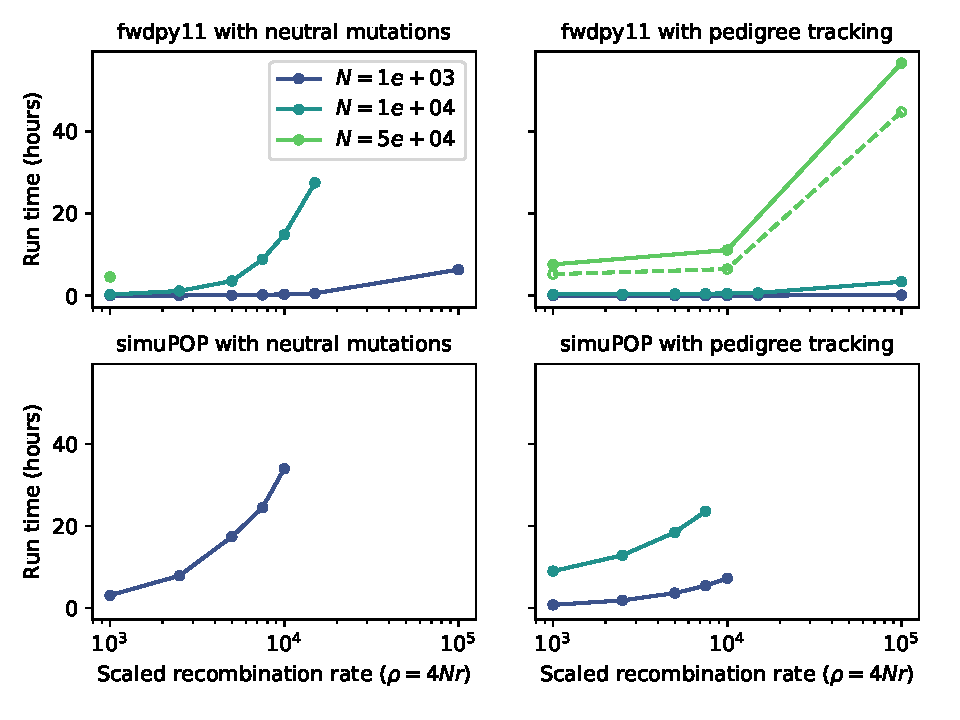
\includegraphics[]{sims/rawspeed}
    \caption{\label{fig:runtimes_selection}Total run time for a single simulation replicate as a function of region
        length, measured as the scaled recombination parameter $\rho = 4Nr$. The different colored lines represent
        different diploid population sizes ($N$). The left column shows run times for
        simulations including the tracking of neutral mutations.  Missing data points are due to either simulations
    being killed at 72 hours or running out of memory (which only happened with \simupop{}).  The right column of
panels shows run times tracking the pedigree instead of the neutral mutations. The dashed line in the upper right panel shows
the results for an implementation using \fwdpy{} where the pedigree simplification steps were handled in a separate thread of
execution and fitness calculations were parallelized.}
\end{figure}

We also performed a more limited set of simulations without natural selection.  The total run times are shown in
Figure~\ref{sfig:rawspeed_nosel} and show the same qualitative behavior as simulations with selection
(Figure~\ref{fig:runtimes_selection}).  The relative improvement due to pedigree tracking is again substantial in these
simulations (Figure~\ref{sfig:speedup_nosel}).  In fact, we see more of a benefit to pedigree tracking here with \fwdpy{}
than we did with selection (Figure~\ref{fig:relative_speedup_selection}).  The reason is that the fitness function exits
close to instantly in simulations without selection that are based on \fwdpp{}, meaning that \fwdpy{} is doing little
more than generating random numbers and book-keeping in Figures~\ref{sfig:rawspeed_nosel}
and~\ref{sfig:speedup_nosel}.


\begin{figure}
    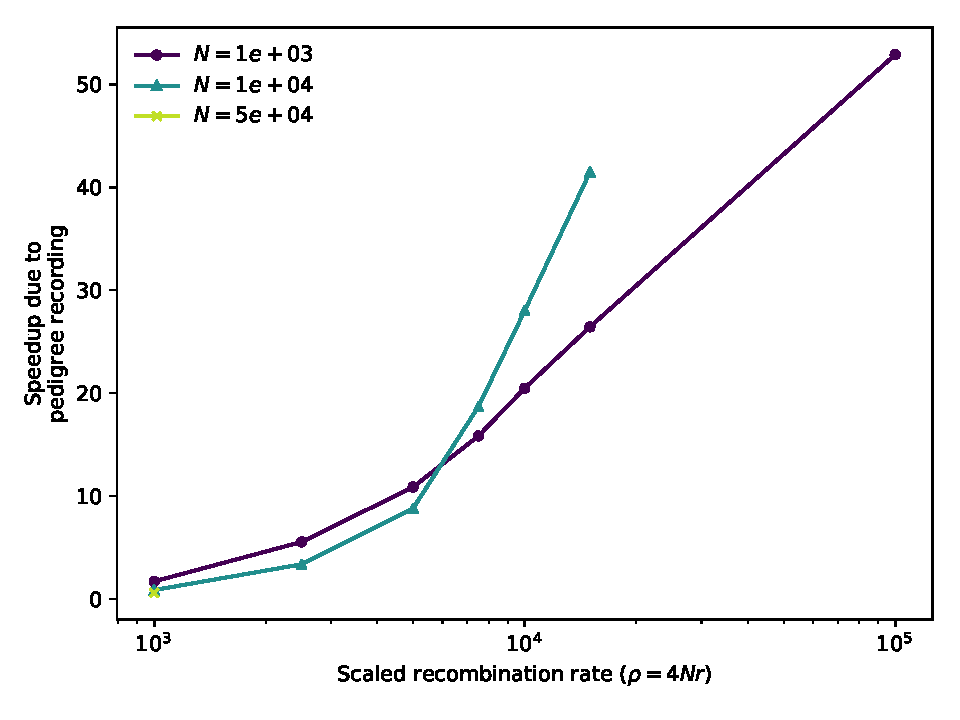
\includegraphics[]{sims/speedup}
    \caption{\label{fig:relative_speedup_selection}Relative performance improvement due to pedigree tracking. This figure
    shows the ratio of the run time tracking neutral mutations over the run time tracking the pedigree. Data points are taken
from Figure~\ref{fig:runtimes_selection} for simulations that ran to completion using both methods.}
\end{figure}

\krt{I should discuss RAM use here}
% Comparison of simulation with/without msprime, using \simupop{}
% or maybe just a simple haploid simulation with 1000 QTL and stabilizing selection on a trait (say).
%
% Maybe an estimate of how long \emph{just} the pedigree recording and simplification takes,
% so that then we can say how fast the simulator would have to be to do $10^6$ whole chromosomes for $10^7$ generations
% in a day.



%%%%%%
\subsection*{Working with a tree sequence through tables}

The simulations above recorded information about each new individual
in collection of tables that together encode a \emph{tree sequence}.
A {tree sequence} is an encoding for a sequence of correlated trees,
such as those describing the history of a sexual population.
A closely related structure is known as the \emph{ancestral recombination graph} --
the {ARG} \citep{griffiths1991two,griffiths1997ancestral},
where nodes are common ancestor or recombination events --
which has been the subject of substantial study
under the assumptions of coalescent
theory~\citep{wiuf1997number,wiuf1999ancestry,marjoram2006coalescent,wilton2015smc}.
However, the properties of the ARG as a computational structure have not
been studied and, despite several efforts to standardise a common
format~\citep{morin2006netgen,mcgill2013graphml}, % TODO check these refs against others in msprime paper.
ARGs are rarely used
in practise. In contrast, the algorithmic properties of tree sequence
algorithms have been explored in detail~\citep{kelleher2016efficient},
contributing substantially to the efficiency of the \msprime\ coalescent simulator.

Tree sequences are efficient because branches that are shared by adjacent trees are stored once,
rather than repeatedly for each tree.
The topology of a tree sequence is defined via its \emph{nodes} and \emph{edges},
while information about variants are recorded as \emph{sites} and \emph{mutations}.
The format for these four tables is given in more detail in the Methods;
here we explain conceptually,
using the example of Figure~\ref{fig:example_tree_sequence}. This formulation
is derived from the ``coalescence records'' encoding of tree
sequences~\citep{kelleher2016efficient}, normalised to remove redundancy
and generalised to include a much larger class of tree topology.

The \emph{nodes} of a tree sequence
correspond to the vertices in the individual genealogies along the sequence,
and each node refers to a distinct ancestor.
Since each node represents a specific ancestor, it has a unique ``time'',
thought of as her birth time, which determines the height of any vertices
she is associated with.
Note that since each node time is equal to the amount of time since the {birth} of the
corresponding parent, time is measured in clock time, not in meioses.
The example of Figure~\ref{fig:example_tree_sequence} has five nodes:
nodes 0, 1 and 2 occur at time 0 and are the \emph{samples},
while nodes 3 and 4 represent those ancestors necessary to record their genealogy,
who were born one and two units of time in the past, respectively.

\begin{figure}
    \begin{center}
        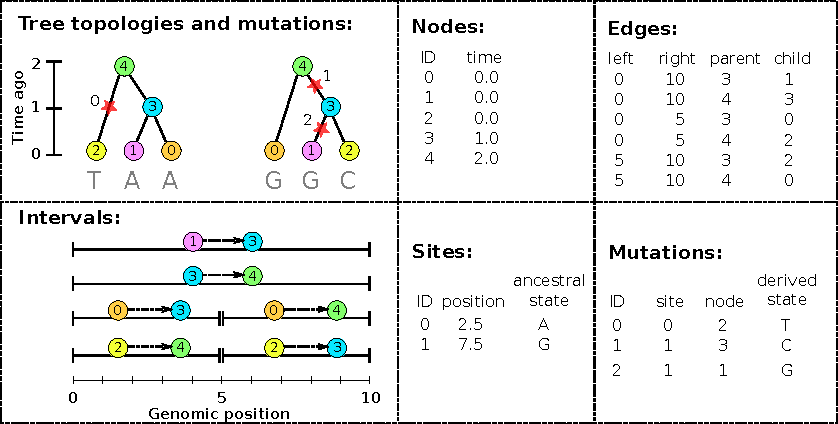
\includegraphics[width=\textwidth]{example_tree_sequence}
    \end{center}
    \caption{
        An example tree sequence with three samples over a chromosome of length 10.
        The left-hand panel shows the tree sequence pictorially in two different ways:
        (top) as a sequence of tree topologies
        and (bottom) the spatial extent of the edges that define these topologies.
        The right-hand panels show the specific encoding
        of this tree sequence in the four tables (nodes, edges, sites and mutations)
        defined by \msprime.
        \label{fig:example_tree_sequence}
    }
\end{figure}

The \emph{edges} define how nodes relate to each other over specific genomic intervals.
Each edge records:
% is a tuple $(\ell, r, p, c)$, where
the endpoints $[\ell, r)$ of the half-open genomic interval defining the
spatial extent of the edge;
and the identities $p$ and $c$ of the parent and child nodes
of a single branch that occurs in all trees covering this interval.
The spatial extent of the edges defining the topology of Figure~\ref{fig:example_tree_sequence}
are shown in the bottom left panel.
For example, the branch joining nodes 1 to 3 appears in both trees,
and so is recorded as a single edge extending over the whole chromosome.
It is this method of capturing the shared structure between adjacent trees that makes the
tree sequence encoding very compact and algorithmically efficient.

Recovering the sequence of trees from this information is straightforward:
each point along the genome that the tree topology changes
is accompanied by the end of some {edges} and the beginning of others.
Since each {edge} records the genomic interval
over which a given node inherits from a particular ancestor,
to construct the tree at a certain point in the genome
we need only retrieve all edges overlapping that point
and construct the corresponding tree.
To modify the tree to reflect the genealogy at a nearby location,
we simply remove those edges whose intervals do not overlap that location,
and add those new edges whose intervals do.
Incidentally, this property that edges naturally encode \emph{differences}
between nearby trees (e.g., as ``subtree prune and regraft'' moves)
allows for efficient algorithms to compute statistics of the genome sequence that take advantage
of the highly correlated nature of nearby trees~\citep{kelleher2016efficient}.

Given the topology defined by the nodes and edges, \emph{sites} and \emph{mutations}
encode the sequence information for each sample in an efficient way. Each site
is associated with a position on the genome and an ancestral state. For example,
in Figure~\ref{fig:example_tree_sequence} we have two sites, one at position
2 with ancestral state `A' and the other at position 7 with ancestral state `G'. If
no mutations occur, all samples inherit the ancestral state at a given site.
Each mutation occurs above a specific node at a given site,
and results in a specific derived state.
Thus, all samples below the mutation's node in the tree will inherit this state,
unless further mutations are encountered.
Three mutations are shown in Figure~\ref{fig:example_tree_sequence},
illustrated by red hexagons.
The first site, in the left-hand tree,
has a single mutation, which results in node $2$ inheriting the state `T'.
The second site, in the right hand tree, has two mutations:
one occurring over node $3$ changing the state to `C',
and a back mutation over node $1$ changing the state to `G'.

This encoding of a sequence of trees and accompanying mutational information is
very concise. To illustrate this, we ran a simulation of 500,000 samples of a
$200$ megabase human-like chromosome ($N_e=10^4$ and per-base mutation and
recombination rates of $10^{-8}$ per generation) using \msprime. This resulted
in about 1 million distinct marginal trees and $1.1$ million infinite-sites
mutations. The HDF5 file encoding the nodes, edges, sites and mutations (as
described above) for this simulation consumed 157MiB of storage space. Using
the \msprime\ Python API, the time required to load this file into memory was
around 1.5 seconds, and the time required to iterate over all 1 million trees
was 2.7 seconds. In contrast, recording the topological information in Newick
format would require around 20 TiB and storing the genotype information
in VCF would require about 1 TiB (giving a compression factor of 144,000 in
this instance).
Working with either the Newick or VCF encoding
of this dataset would likely require several
days of CPU time just to read the information into memory.

\paragraph{Validity of a set of tables}
Given a set of node and edge tables as described above,
there are only two requirements that ensure the tables
describe a valid tree sequence.
% (There are essentially no such requirements on the site and mutation tables.)
These are:
\begin{enumerate}
    \item Offspring must be born after their parents (and hence, no loops).
    \item The set of intervals on which each individual is a child must be disjoint.
\end{enumerate}
A pair of node and edge tables that satisfy these two requirements
is guaranteed to uniquely describe at each point on the genome
a collection of directed, acyclic graphs -- in other words, a forest of trees.
For some applications it is necessary to check that at every point
there is only a \emph{single} tree.
Checking this is more difficult, but is implemented in \msprime{}'s API.
% \jda{TODO add function name}  PLR: not sure this is necessary.
For efficiency, \msprime{} makes several other sortedness requirements on the tables,
that are not necessarily satisfied by tables emitted by a forwards-time simulation.
\msprime{}'s API includes tools to rectify this by first sorting % (using \texttt{sort\_tables})
and then using the \texttt{simplify} algorithm described below, which works on sorted tables
and is guaranteed to produce a valid, \msprime{}-ready tree sequence.


%%%%%%
\subsection*{Recording the pedigree in forwards time}

To record the genealogical history of a forwards in time simulation
we need to record two things for each new chromosome:
the birth time, and the endpoints and parental IDs of each distinctly inherited segment,
which are naturally stored as the \emph{nodes} and \emph{edges} of a tree sequence.
For concreteness, we write out in pseudocode how to run a neutral Wright--Fisher simulation
that records genealogical history in this way.
The simulation will run for $T$ generations,
and has $N$ haploid individuals, each carrying a single chromosome of length $L$.
For simplicity, we sample exactly one crossover per generation.

We use $\randomuniform(A)$ to denote an element of the set $A$ chosen uniformly at random
(and all such instances are independent).
Given a node table $\Nt$, the function $\taddnode{\Nt, t}$
adds a new node to the table $\Nt$ with time $t$
and returns the ID of this new node.
Similarly, the function $\taddedge{\Et, \ell, r, p, c}$
adds a new edge $(\ell\mathrm{eft}, r\mathrm{ight}, p\mathrm{arent}, c\mathrm{hild})$ to the edge table $\Et$.
The function $\tsimplify{P, \Nt, \Et}$ (described in section \ref{ss:simplify})
simplifies the history stored in the tables $\Nt$ and $\Et$
to the minimal information required to represent the genealogies of the list of node IDs $P$;
after simplification the nodes appearing in $P$ are relabeled $(0, 1, \ldots, |P|)$.
A step-by-step explanation follows the pseudocode.

\begin{taocpalg}{W}{Forwards-time tree sequence}
{Simulates a randomly mating population of $N$ haploid individuals with
chromosome of length $L$ for $T$ generations, and returns the node
and edge tables ($\Nt$ and $\Et$) recording the simulated history.
The tables are simplified every $s$ generations, removing genealogical
information from $\Nt$ and $\Et$ unreachable from the current population $P$.
}

\algstep{W1.}{Initialisation.}{
Set $\Nt \leftarrow \mbox{NodeTable}()$, $\mathcal{E}
\leftarrow \mbox{EdgeTable}()$, $t \leftarrow T$, and $j \leftarrow 0$.
 For $0 \leq k < N$, set $P_k \leftarrow \taddnode{\Nt, T}$.
}

\algstep{W2.}{Generation loop head: new node.}{Set $u \leftarrow \taddnode{\Nt, t}$ and $P'_j \leftarrow u$.
}

\algstep{W3.}{Choose parents.}{Set $a \leftarrow \randomuniform(\{0, \dots, N - 1\})$,
    $b \leftarrow \randomuniform(\{0, \dots, N - 1\})$ and $x \leftarrow \randomuniform([0, L))$.
}

\algstep{W4.}{Record edges}{
Call $\taddedge{\Et, 0, x, P_a, u}$ and $\taddedge{\Et, x, r, P_b, u}$.
}

\algstep{W5.}{Individual loop}{Set $j \leftarrow j + 1$. If $j < N$ go to \algref{W2}.
Otherwise, if $t\bmod s \neq 0$ go to \algref{W7}.
}

\algstep{W6.}{Simplify.}{Call $\tsimplify{P', \Nt, \Et}$, and set $P'_k
\leftarrow k $ for $0 \leq k < N$. (Tables may need to be sorted.)}

\algstep{W7.}{Generation loop.}{Set $t \leftarrow t - 1$. If $t = 0$ terminate.
Set $P \leftarrow P'$, $j \leftarrow 0$, and go to \algref{W2}.
}

\end{taocpalg}

We begin in~\algref{W1} by creating new node and edge tables, and setting
our population $P$ (a vector of $N$ node IDs) to the initial population.
This initial population is a set of $N$ nodes with birth time $T$ generations
ago. We also initialise our generation clock $t$ and individual index $j$.
Steps~\algref{W2}--\algref{W4} replace the individual with node ID
$P_j$ by first creating a new node with birth time $t$ (and ID $u$).
In step~\algref{W3} we choose two indexes $a$ and $b$ uniformly,
giving us parental IDs $P_a$ and $P_b$,
and choose a chromosomal breakpoint $x$.
We record the effects of this event by storing two new edges: one recording that the parent of node $u$
from $0$ to $x$ is $P_a$, and another recording that the parent of $u$
from $x$ to $L$ is $P_b$. Step \algref{W5} then iterates these steps
for each of the $N$ individuals for each generation.
At the end of a generation, we then check
if we need to simplify (which is done every $s$ generations).
If simplification is required, we do this in step \algref{W6} by calling the simplify function
on the node and edge tables with the current set of population IDs $P'$ as the samples.
This updates the tables in-place to remove all redundant
information, and remaps the specified sample IDs to $0, \dots, N - 1$ in the updated tables.
Hence, we set our current population IDs to
$0, \dots N - 1$ after simplify has completed.
Step \algref{W7} loops these steps until the required number of generations have been simulated.
% then completes the algorithm by looping over generations;
% we decrement our clock $t$, and terminate if $t = 0$.
% Otherwise, we update our current population and individual index and loop
% back to \algref{W2}.


\begin{figure}
    \begin{center}
        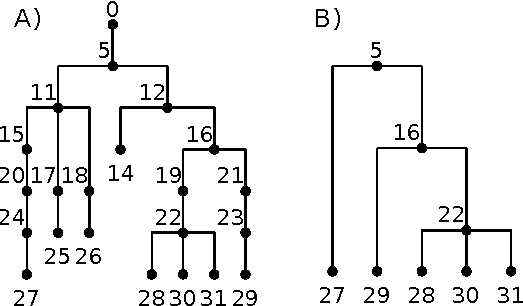
\includegraphics{wf-before-after}
    \end{center}
    \caption{An example of a marginal genealogy from a Wright-Fisher simulation
    with $N=5$. \textbf{(A)} the original tree including all
    intermediate nodes and dead-ends, and \textbf{(B)} the minimal tree
    relating all of the currently-alive individuals (27--31).
    \label{fig:wf-trees}
    }
\end{figure}


\krt{The following paragraph has a sentence mangling.  I think some comment is warrented about when it is useful to
record selected mutations, like for ancient samples?}

This algorithm records only topological information about the simulated genealogies,
but it is straightforward to add mutational information.
This can be done in two different ways.
We can record mutations that occur during the simulation by simply
randomly sampling new mutations after recording the edges joining the new node $u$ to its parents
$P_a$ and $P_b$ in step \algref{W7}.
It is straightforward to record this information during the simulation, but it
Alternatively, we can generate these mutations after the simulation has completed, thus
avoiding the cost of generating the many mutations that are lost in the population.
This is straightforward to do because we have access to the marginal genealogies.

Figure~\ref{fig:wf-trees} shows
an example of a marginal genealogy produced by a forwards-time Wright--Fisher
process like Algorithm~\algref{W}.
On the left is the tree showing all the edges output by the simulation,
while on the right
is the minimal tree representing the ancestry of the currently alive population.
Clearly there is a great deal of redundancy in the topological
information output by the simulation.
This redundancy comes from two sources.
First, there are a large number of nodes in tree that have only one child.
In Algorithm~\algref{W} we do not attempt to identify coalescence events,
but simply record all parent-child
relationships in the history of the population.
As such, many of these edges
will record the simple passing of genealogical information from parent to child
and only some small subset will correspond to coalescences within the marginal
trees. The second source of redundancy in the output of Algorithm~\algref{W}
is due to the fact that lineages die out: a large number of
individuals in the simulation leave no descendants in the present day population.
Node 26 in Figure~\ref{fig:wf-trees}a, for example, leaves no
ancestors in the current population, and so the entire path tracing back to
the root is redundant.

%%%%%%
\subsection*{Tree sequence simplification}
\label{ss:simplify}

It is desirable for many reasons to remove redundant information from a tree sequence,
such as those produced by a forwards-time simulation.
To formalize this:
suppose that we are only interested in a subset of the nodes of a tree sequence
(which we refer to as our `samples'),
and wish to reduce this input tree sequence
into the minimum representation of the topologies that include the specified samples.
The output tree sequence must have the following properties:
\begin{enumerate}
\item All marginal trees must match the subtree induced by the samples of the corresponding tree in the input tree sequence.
\item Within the marginal trees, all non-sample vertices must has at least
two children (i.e., unary tree vertices are removed).
\item Any nodes and edges not ancestral to any of the sampled nodes are removed.
\item There are no adjacent redundant edges, i.e., pairs of edges
    $(\ell, x, p, c)$ and $(x, r, p, c)$ which can be represented with a single edge
    $(\ell, r, p, c)$.
\end{enumerate}


\begin{figure}
    \begin{center}
        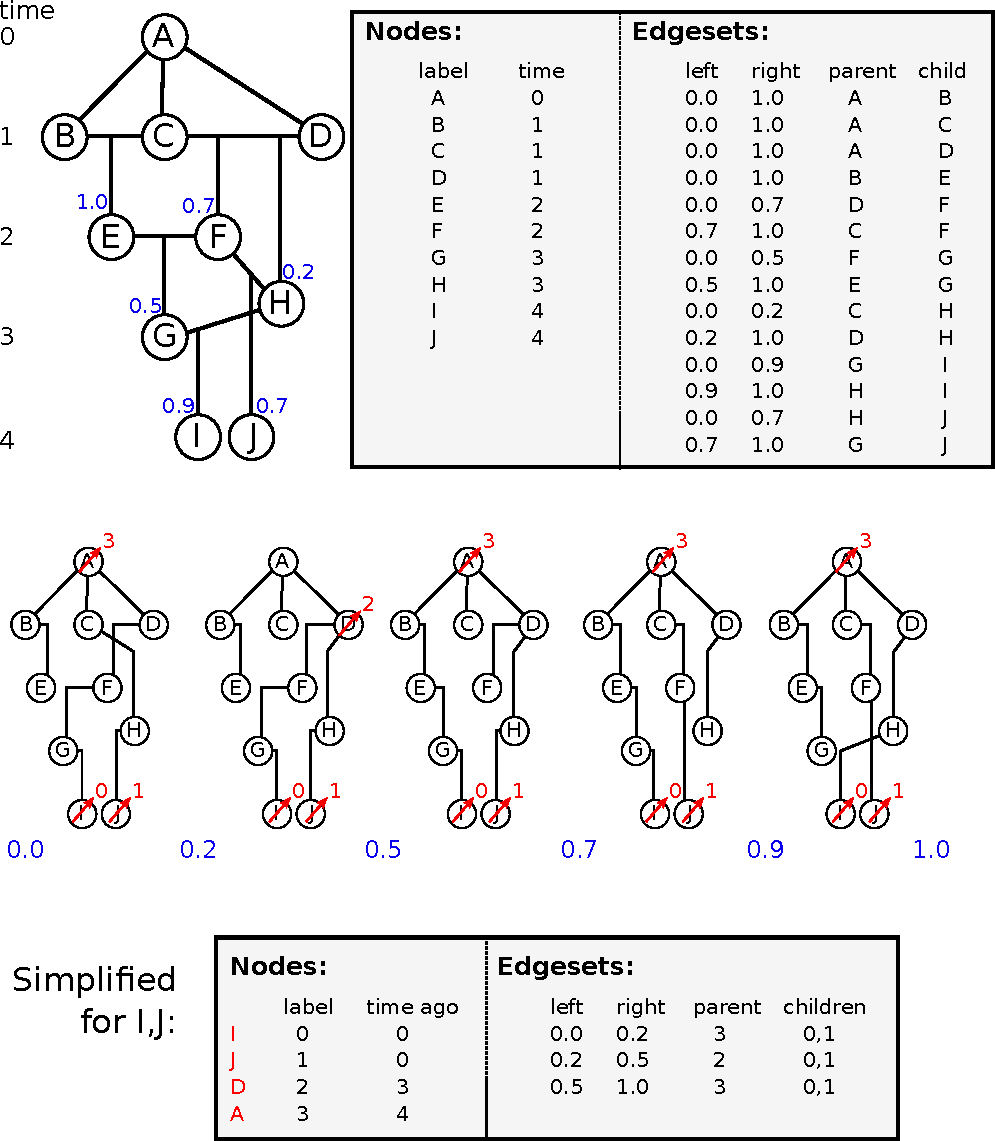
\includegraphics{method_diagram}
    \end{center}
    \caption{
        A simple example of the simplify method.
        \textbf{Top:} the diagram on the left relates ten haploid individuals to each other.
        It has 10 node records (one for each individual)
        and 14 edge records (one for each distinctly inherited segment).
        Blue numbers denote crossing over locations in each meiosis --
        for instance, $C$ and $D$ were parents to $F$,
        who inherited the left 70\% of the chromosome from $D$ and the remainder from $C$.
        The individuals $B$, $C$, and $D$ inherit clonally from $A$.
        \textbf{Center:} the five distinct trees relating all individuals to each other
        found across the chromosome (blue numbers denote locations on the chromosome).
        Labels after simplification are shown in red.
        \textbf{Bottom:} tables recording the tree sequence after simplification
        with nodes $I$ and $J$ as samples.
        The mapping from labels in the forwards time simulation to nodes in the tree sequence
        is shown in red.
        % which allows additional records to be added as the simulation progresses.
        \label{fig:method_diagram}
    }
\end{figure}

Simplification is essential
not only for keeping the information recorded by forwards simulation manageable,
but also is useful for extracting subsets of a tree sequence representing a very large dataset.
% The tree sequences produced by forwards simulations
% record all of history for everyone alive at any time through the simulation.
% Simplification is essential to reduce this
% to a manageable quantity that still contains all
% the information that we are interested in.
% Simplification is also useful if we have a
% tree sequence representing a large dataset and wish to extract the
% information relevant to a subset of the samples.

Our approach to simplification is based on Hudson's algorithm for simulating
the coalescent with recombination~\citep{hudson1983properties},
paralleling the implementation in \msprime{} \citep{kelleher2016efficient};
an implementation in pseudocode is provided in Appendix~\ref{ss:simplify_algorithm}.
Conceptually, this works by
(a) beginning by painting the chromosome each sample a distinct color;
(b) moving back through history,
copying the colors of each chromosome to the portions of its' parental chromosomes
from which it was inherited;
(c) each time we would paint two colors in the same spot (a coalescence),
record that information as an edge and instead paint a brand-new color;
and
(d) once all colors have coalesced on a given segment,
stop propagating it.
This ``paint pot'' description misses some details --
for instance, we must ensure that all coalescing segments in a given individual
are assigned the \emph{same} new color --
but is reasonably close.
Figure~\ref{fig:method_diagram} shows an example tree sequence,
before and after simplification,
and Figure~\ref{fig:simplify_state} depicts the ``paint pot'' state of the algorithm
during the process of simplifying this tree sequence.

\begin{figure}
    \begin{center}
        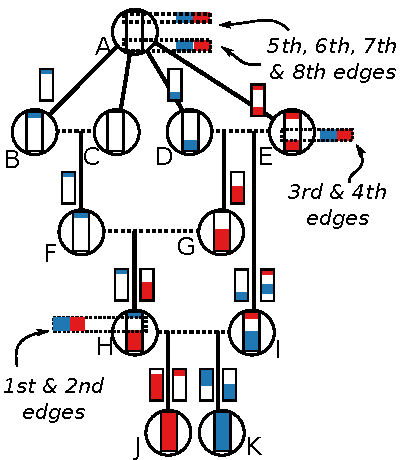
\includegraphics{simplify-state-diagram}
    \end{center}
    \caption{
        A depiction of the state of the simplification algorithm
        at each point in time,
        in the example of Figure~\ref{fig:method_diagram}.
        \label{fig:simplify_state}
    }
\end{figure}

More concretely,
the algorithm works by moving back through time,
processing each parent in the input tree sequence in chronological order.
The main state of the algorithm at each point in time is a set of ancestral lineages,
and each lineage is a linked list of ancestral segments.
An ancestral segment $(\ell, r, u)$ is found in a lineage
if the output node $u$ inherits the genomic interval $[\ell, r)$ from that lineage
(and so $u$ corresponds to a ``color'' in the description above).
% These segments are stored in a collection of linked lists,
% one list of segments for each ancestral lineage present at that time.
We also maintain a map $A$ such that $A_j$ is the lineage
corresponding to node $j$ in the input tree sequence.
Crucially, the time required to run the algorithm is
linear in the number of edges of the input tree sequence.

%%%%%%%%%%%%%%
\subsubsection*{Sequential simplification and prior history}

Any simulation scheme that records data into tables,
as does Algorithm~\algref{W},
has its genealogical history available at any time as a tree sequence.
This has two additional advantages:
First, simplification can be run periodically through the simulation,
if we take the set of samples to be the entire currently alive population.
This is important in practice as it keeps memory usage from growing linearly (and quickly) with time.
Second, the simulation can
be \emph{begun} with a tree sequence produced by some other method -- for
instance, by a coalescent simulation with \msprime,
providing an easy, efficient way to specify prior history.
A natural question is now: how often should simplification occur?
As shown in the next section,
there is no computational advantage to simplifying more often than is necessary
to keep memory usage down.



%%%%%%%%%%%%
\subsubsection*{Estimates of run-time complexity}

\plr{Refer to simulation results here.}

%% Memory reduction thanks to simplification
Consider a simulation of a Wright-Fisher population of $2N$ haploid individuals
using Algorithm~\algref{W} for $T$ generations,
with simplify interval $s = 1$ so that redundant information is removed after every generation.
Since every chromosome inherits material from both parents,
without simplification this would produce tables of
$2NT$ nodes and
$4NT$ edges.
Suppose that $T$ is large enough that all samples coalesce within the simulation with high probability,
($T \sim 20N$, say).
After simplification, we are left with the tree sequence describing the history
of only the current generation of $2N$ individuals.
This tree sequence has $4N-2$ edges to describe the leftmost tree;
and each time the marginal tree changes along the sequence,
four edges end and four new edges begin
(except for changes affecting the root, which require fewer; see \citet{kelleher2016efficient}).
Coalescent theory tells us that
the expected total length of the edges of a marginal tree is approximately $4N\log(2N)$,
which is also equal to the mean number of ancestral recombination events that occur on a branch of the marginal tree,
since we have taken one crossover per individual per generation.
Not all such recombinations actually change the tree topology,
so four times this gives us an upper bound on the expected number of additional edges.
Similarly, not every new edge derives from a never-before-seen node,
but the number of nodes is at most equal to the number of edges plus the sample size.
With $T=20N$, this reduces the initial storage of $120 N^2$ items to
% 4N - 2 + 2N + 4N log(2N) * 4 * 2 = 6N + 32 N log(2N)
$6N + 32 N \log(2N)$;
at $N=10^4$, a factor of 3,700.

%% Progressive memory reduction as a function of T
To get an idea of how required space depends on the length of time between simplification steps,
suppose instead that we have run a simulation of $2N$ individuals for $T$ generations,
begun with no prior history.
How many of the resulting $4NT$ edges are required after simplification?
As above, the expected number of edges is bounded by $2N-2$ plus four times the mean marginal tree length.
Roughly, the length of time for which a marginal tree has $k$ tips is
$2N/k(k-1) = 2N(1/(k-1) - 1/k)$,
and so the time to go from $N$ to $n$ tips is $2N(1/(n-1) - 1/(N-1))$.
This implies that after running for time $T$ we expect to
have around $n(T)$ roots, where $n(T) \approx 1 + 2N/(T+2)$.
The total tree length over this time is
$2 N \sum_{k=n(T)+1}^{N-1} 1/k$, which
% is approximately
% \begin{align*}
%     2 N \log\left( \frac{N}{1 + 2 N/(T+2)} \right) .
% \end{align*}
leads to an upper bound on the number of edges of
\begin{align}
    \label{eqn:edge_bound}
    2 N \left( 1 + 4 \log\left( \frac{NT}{T + 2 N} \right)\right) .
\end{align}
This holds up quite well in practice,
as shown in Figure~\ref{fig:simplify_complexity}.
% by comparison to
% the number of edges actually required for 50 independent Wright--Fisher simulations,
% as a function of time (obtained from Algorithm~\algref{W} with $s=1$)
% is shown in Figure~\ref{fig:simplify_complexity}, compared to this prediction.

\begin{figure}
    \begin{center}
        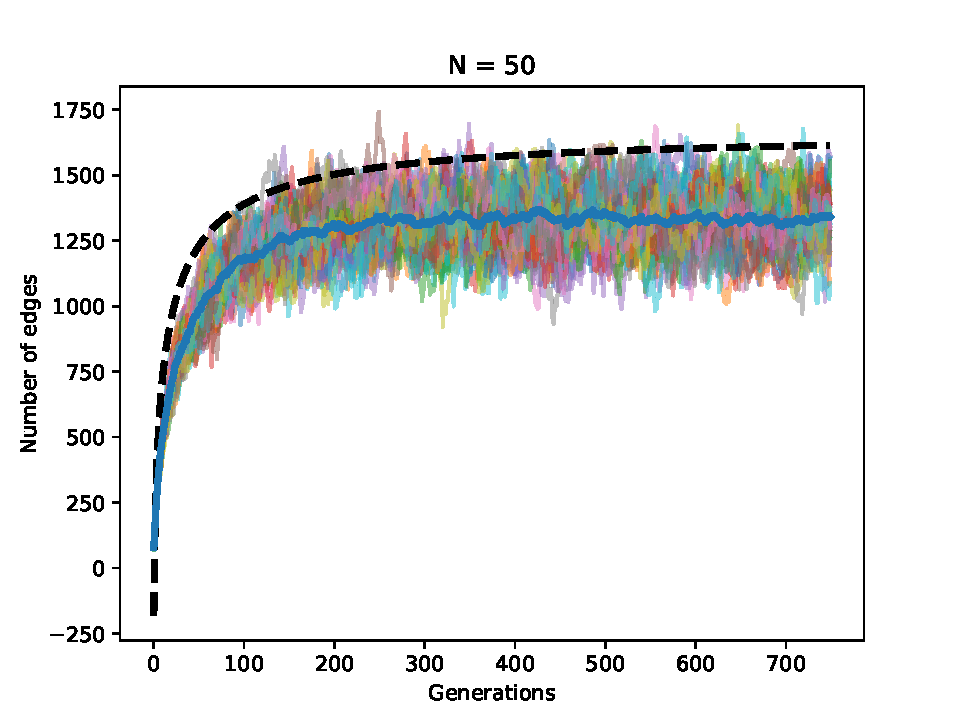
\includegraphics{sims/num_edges_50}
        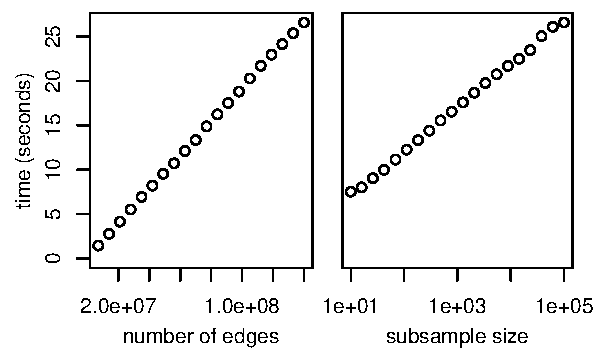
\includegraphics{sims/simplify_timings}
    \end{center}
    \caption{
        \textbf{(A)}
        Number of edges in the simplified tree sequence
        for 50 Wright--Fisher simulations begun with no prior history,
        as a function of number of generations.
        Each line is one simulation, the black line gives the average,
        and the dotted line is the upper bound of equation \eqref{eqn:edge_bound}.
        \plr{Propose to add other figures as subfigures here; but better than this.}
        \textbf{(B)}
        Time required to simplify the first $k$ edges
        of \plr{what tree sequence?},
        plotted against $k$.
        \textbf{(C)}
        Time required to simplify
        \plr{what tree sequence?}
        down to a sample of size $n$,
        plotted against $n$
        (note the log scale;
        the time scales logarithmically with $n$).
        \label{fig:simplify_complexity}
    }
\end{figure}

%% Above was edges; same holds for memory usage savings due to mutations
If we were to add mutations in forwards time
under the infinite-sites model with total mutation rate per generation $\mu$,
there would also be around $\mu 2NT$ mutations (and the same number of sites).
Since mutations fall as recombinations do on the marginal trees,
adding them after simplification results in only around $\mu 4 N \log(2N)$ mutations,
and the same savings as we obtained from edges above,
even without considering the
computational burden of propagating mutations forwards across generations.


%% simplify run time
Above we have described memory requirements;
how does the computation time required for simplification scale?
Simply because it must process each edge,
the simplification algorithm is linear in the number of edges of the input tree sequence.
This is seen in Figure~\ref{fig:simplify_complexity}X,
where we show shows the time required to simplify increasingly large subsets of a large tree sequence.
When simplifying the result of a forwards-time sequence, the number of edges is the main contributing factor.
Suppose on the other hand we want to
simplify an already-minimal but large tree sequence with $N$ nodes
to a subsample of size $n$.
How does the required time scale with $n$?
In this case, the computation is dominated by the size of the output tree sequence,
which grows with $\log(n)$.
this is also seen in Figure~\ref{fig:simplify_complexity}X,
showing the time required to simplify progressively larger subsets of a single large tree sequence.


Our method stores genealogies, and so records substantially more information
than would a method only recording genotypes.
However, since the simplification algorithm requires computational effort,
it is informative to compare computational complexity of the algorithm
to one that propagates neutral genotypes.
A typical individual differs at around $2 N \mu$ sites from the population's consensus sequence,
so propagating these to offspring by simple copying will take $4 N^2 \mu$ operations per generation.
On the other hand,
in our scheme we must store $13N$ quantities per generation (two edges and one node per individual).
\plr{XXX}
The simplification algorithm is linear in the number of edges of the input tree sequence
(because it must process each edge),
and so multiplies this by a constant factor.
This implies that propagating neutral genotypes for $T$ generations has time complexity $O(\mu T N^2)$,
while our implementation is only $O(T N \log(2N))$.


%%%%%%
\subsection*{Overview of the API}

These tools are implemented through the \msprime{} Python API,
which provides a powerful platform for working with tree topology and mutation data.
The new portions of \msprime{} that we cover here
are dedicated to tree sequence input and output using simple tables of data,
so we refer to this as the `Tables API'.
The four key tables: nodes, edges, sites and mutations, are described above.

The Tables API is primarily designed to facilitate efficient interchange of
data between programs or between different modules of the same program.
% we are capitalizing Tables API but not the more generic "tables".
% \jda{should capitalize Tables, or not, as above}
Following current best practises
\plr{citations: Apache arrow, etc},
data is stored in a columnar format,
which allows for very efficient interchange of large amounts of numerical data.
In principle, this enables zero-copy semantics,
where a data consumer can read the information directly
from the memory of a producer without incurring the overhead of a copy.
Our implementation uses the numpy C API \citep{numpy_C_api} to efficiently copy
data from Python into the low-level C library used to manipulate tree sequences.
Since tables are encoded as contiguous arrays of numeric data,
this achieves data transfer rates that would be impossible under
any text-based approach while retaining excellent portability.

This also provides basic input and output operations via numpy's
array interface, which provides a great deal of flexibility and efficiency,
and makes it straightforward to transfer data from sources
such as HDF5 \citep{hdf5}, Dask, or Zarr.
(For small scale data and debugging purposes, a simple text format is also supported.)
% PLR: this was mentioned above, and belongs in the documentation, I think.
% The API also provides functions to sort tables
% to ensure that the records are in the form required to input
% into an \msprime{} tree sequence object. (Simplification may also be required.)

The \msprime{} Tables API is designed to be easily ``plugged'' into any simulation engine.
One simply needs to fill the relevant columns,
and to send them to \msprime{} at regular intervals for simplification.
For example, in the benchmarking simulations above,
we used the \fwdpp{} C++ API \citep{fwdpp}
to fill arrays of simple structures representing the node and edge data.
Doing so requires no modification of the \fwdpp{} code base.
Rather, we simply need to bookkeep parent/offspring labels,
and perform simple processing of the recombination breakpoints from each mating event.
Using \texttt{pybind11} (\url{https://github.com/pybind/pybind11/}),
the node/edge arrays on the C++ side are made visible, without copy, to Python as a multi-column numpy array,
which is processed by the \msprime{} tables API.
Our implementation also uses \texttt{pybind11}
to create a Python package extending \texttt{fwdpy11}
(a Python package based on \fwdpp{}; \url{https://github.com/molpopgen/fwdpy11}),
% (A neat aside, that we may wish to skip here, is that it may be possible to use the tables
% API from a command-line C/C++ application via an embedded Python interpreter.)



%%%%%%%%%%%%%%%%%%%%%%
\section*{Discussion}

In this paper, we have shown that storing pedigrees
and associated recombination events
in a forwards-time simulation
not only results in having available a great deal more information about the simulated population,
but also can speed up the simulation by orders of magnitude.
To make this feasible,
we have described how to efficiently store this information in numerical tables,
and have described a fundamental algorithm for simplification of tree sequences.
Conceptually, recording of genealogical and recombination events
can happen independently of the details of simulation;
for this reason, we provide a well-defined and well-tested API in Python
for use in other code bases (a C API is also planned).

The idea of storing genealogical information to speed up simulations is not new.
It was implemented completely in AnA-FiTS~\citep{aberer2013rapid},
but without the critical step of discarding irrelevant genealogical information.
A similar but much more limited method for
discarding this information does appear in \citet{padhukasahasram2008exploring}.


The tree sequences produced by default by this method
are very compact, storing genotype \emph{and} genealogical information
in a small fraction of the space taken by a compressed VCF file.
The format is also highly efficient to process,
leading to advantages for downstream analysis as well.
This is because many algorithms to compute statistics of interest for population genetics
are naturally expressed in terms of tree topologies,
and so can be quickly computed from the trees underlying the tree sequence format.
For example, pairwise nucleotide diversity $\pi$, is the average density of
differences between sequences in the sample.
To compute this directly from sequence data at $m$ sites in $n$ samples
requires computing allele frequencies, taking $O(nm)$ operations.
By using the locations of the mutations on the marginal trees,
and the fact that these are correlated,
sequential tree algorithms similar to those in~\citep{kelleher2016efficient}
can do this in roughly $O(n + m \log n)$ operations.
The \msprime{} API provides a method to compute $\pi$ among arbitrary subsets of the
samples in a tree sequence, which took about 1.2 seconds
applied to the example tree sequence above with 1.1 million mutations
in 200 megabases for 500,000 samples.
Calculating $\pi$ from the numeric genotype matrix using numpy took \plr{HOW MANY} seconds.

Another attractive feature of this set of tools
is that it makes it easy to incorporate \emph{prior history},
simply by seeding the simulation with a (relatively inexpensive) coalescent simulation.
This allows for incorporation of deep-time history beyond the reach of individual-based simulations.
This may not even negatively affect realism,
since geographic structure from times longer ago than the mixing
time of migration across the range has limited effect on modern genealogies
\citep{wilkins2004separation},
other than possibly changing effective population size \citep{barton2002neutral,cox2002stepping}.

Simulating very large populations and entire genomes will likely require parallelization.
The one-way nature of information flow here makes our scheme relatively easy to incorporate
into a parallel algorithm.
Recently, \citet{lawrie2017accelerating} used parallelization
to improve performance for the ``Poisson Random Field'' family of models~\citep{Sawyer1992-jw},
in which mutations are unlinked and there is no effect of genetic background on fitness.
However, thus far little attention has been paid to parallelization of simulations involving linkage.

A final note:
in preparing this manuscript,
we debated a number of possible terms for the embellished pedigree,
i.e., the ``pedigree with ancestral recombination information''.
Etymological consensus \citep{liberman2014little} has
``pedigree'' derived from the french ``pied de grue'' for the foot of a crane
(whose branching pattern resembles the bifurcation of a single parent-offspring relationship).
An analogous term for the embellished pedigree might then be \emph{nedigree},
from ``nid de grue'',
as the nest of a crane is a large jumble of (forking) branches.
We thought it unwise to use this term throughout the manuscript,
but perhaps it will prove useful elsewhere.


%%%%%%%%%%%%%%
% \section*{Methods}


%%%%%%%%%%%%%%%%%%%%%%
\section*{Acknowledgements}
Thanks to Brad Shaffer and Evan McCartney--Melstad for useful discussions.
Funding for this project came from XXX


\bibliography{references}

\appendix

%%%%%%%%%%%%%%
\section{Simplification algorithm}
\label{ss:simplify_algorithm}

\plr{Replace this with Jerome's interval-tree implementation?}

Here we describe the simplification algorithm.
The flow is close to our implementation,
but the description below uses set operations,
while in the implementation,
all ancestors are maintained as linked lists of segments
ordered by left endpoint.
As it goes, the algorithm
records a list $M$ that gives the mapping
from input nodes to output nodes,
so that if $M[p] = u$ then the $p^\text{th}$ node in the input
is the same as the $u^\text{th}$ node in the output.
The current state of the algorithm is recorded in $\Al$,
a list of ancestors
each of which is a collections of ancestral segments.
An ancestral segment is a triple $(\ell, r, x)$,
indicating that the output node $x$ inherits from this ancestor
on the genomic segment $[\ell, r)$.

\begin{taocpalg}{S}{Simplify a tree sequence}
{Input consists of
    a list $S$ of sample IDs,
    a list $\Nt_I$ of nodes (ordered by birth time),
    a list $\Et_I$ of edges,
    and the genome length, $L$.
    The output is a
    nodes $\Nt_O$,
    and list of edges $\Et_O$.
}

\algstep{S0.}{Initialize.}{
    Set $\Al[j] \leftarrow (0, L, j)$
    and $\Nt_O[j] \leftarrow \Nt_I[S[j]]$ for $0 \le j < \len(S)$.
    Set the current input parent index to $p=0$
    and $M[u] \leftarrow -1$ for $0 \le u < \len(\Nt_I)$.
}

\algstep{S1.}{Input parent loop.}{Set $Q \leftarrow \emptyset$.
}

\algstep{S2.}{Remove ancestry.}{Call Algorithm \algref{R} on each edge $(\ell, r, p, c)$ in $\Et_I$
    corresponding to parent $p$ (which stores the resulting segments in the merge queue $Q$).
}

\algstep{S3.}{Merge ancestors.}{Call Algorithm \algref{M} on $Q$
    (which adds to $\Nt_O$ and $\Et_O$).
}

\algstep{S4.}{Next parent.}{Set $p \leftarrow p+1$;
    if $p = \len(\Nt_I)$, terminate and return $\Nt_O$ and $\Et_O$;
    otherwise, return to \algref{S1}.
}

\end{taocpalg}

The algorithm steps back up through the pedigree,
since nodes are ordered by time-since-birth.
First, for each input node $p$, we must find all ancestral segments inheriting from $p$ --
so, for every edge $(\ell, r, p, c)$,
Algorithm \algref{R} replaces any ancestry segment $[u, v)$ held by $c$
with $[u,v) \setdiff [\ell, r)$
(deleting the segment or splitting in two if necessary),
and adding the removed segment $[u,v) \cap [\ell, r)$ to the merge queue $Q$:

\begin{taocpalg}{R}{Remove ancestry}
    {Given an edge $(\ell, r, p, c)$,
    and a list $\Al[c]$ of the $m$ ancestral segments corresponding to $c$,
    remove segments overlapping $[\ell, r)$ from $\Al[c]$,
    and add those overlapping segments to $Q$.
    }

    \algstep{R0.}{Initialize.}{
        Set $j \leftarrow 0$.
    }

    \algstep{R1.}{Segment loop.}{
    If $j=m$, terminate; else let $(u, v, x) = \Al[c][j]$.
    (Here $x$ is the output node that inherits from this segment.)
    }

    \algstep{R2.}{Add to merge queue.}{If $[u,v) \cap [\ell,r) = \emptyset$,
    skip to \algref{R4}.
    Otherwise, append $(\max(u,\ell), \min(v,r), x)$ to $Q$.
    }

    \algstep{R3.}{Remove ancestry.}{
    Delete $\Al[c][j]$ and insert in its place
    $(\min(u,\ell), \max(v,\ell), x)$ (if $u<\ell$)
    and(/or) $(\min(v,r), \max(v,r), x)$ (if $r<v$).
    }

    \algstep{R4.}{Iterate.}{Set $j \leftarrow j+1$ and return to \algref{R1}.
    }

\end{taocpalg}

Next we must merge the ancestry segments in $Q$,
creating the new ancestor corresponding to input node $p$,
adding a node and edges to the output if any segments overlap,
which implies that an output coalescence has occurred.
Below we index elements of an ancestral segment $z = (\ell, r, u)$
by writing $z.\lleft = \ell$ and $z.\lright = r$ for the endpoints,
and $z.\lid = u$ for the output node ID.

\begin{taocpalg}{M}{Merge ancestors}
    {Merge the ancestral segments in $Q$,
    and create the new ancestor $\Al[p]$.
    This algorithm also appends to $\Nt_O$ and $\Et_O$,
    and needs to know about $S$,
    to check if input nodes are samples.
    }

    \algstep{M0.}{Initialize.}{
        Set $z \leftarrow (0, 0, -1)$ and $d = \text{False}$.
    }

    \algstep{M1.}{Segment loop.}{If $\len(Q) = 0$, go to \algref{M9}.}

    \algstep{M2.}{Find next segment overlap boundaries}{
        Let $\ell_0 \leftarrow \min\{x.\lleft : x \in Q\}$
        and $H \leftarrow \{x \in Q : x.\lleft = \ell_0\}$.
        Also let $\ell_+ \leftarrow \min\{x.\lleft : x \in Q \setdiff H\}$
        and $r = \min(\ell_+, \min\{x.\lright : x \in H\})$.
    }

    \algstep{M3.}{Copy single segment.}{
        If $\len(H) = 1$,
        set $\alpha \leftarrow (\ell, r, H[0].\lid)$.
        If also $p \in S$, then
        set $\alpha.\lid \leftarrow M[p]$ and
        $\add(\Et_O, (\alpha.\lleft, \alpha.\lright, \Nt[p], \alpha.\lid))$.
        Go to \algref{M7}.
    }

    \algstep{M4.}{New output node.}{
        If $M[p] = -1$ set $M[p] \leftarrow \add(\Nt_O, \Nt_I[p])$
        Set $\alpha \leftarrow (\ell, r, M[p])$.
    }

    \algstep{M6.}{Record edges and update $Q$.}{
        For each $x \in H$, do $\add(\Et_O, (\ell, r, M[p], x.\lid))$.
    }

    \algstep{M7.}{Update $Q$.}{
        Remove from $Q$ any segment $x \in H$ with $x.\lright = r$
        and then set $x.\lleft = \ell$ for all remaining $x \in H$.
    }

    \algstep{M8.}{Add segment to ancestor.}{
        If $z.\lright = \alpha.\lleft$ and $z.\lid = \alpha.\lid$ set $d = \text{True}$.
        Append $\alpha$ to $\Al[p]$, set $z \leftarrow \alpha$, and return to \algref{M1}.
    }

    \algstep{M9.}{Defragment.}{
        If $d$ is True, find and merge any adjacent segments in $\Al[p]$
        with the same $\lid$.  Terminate.
    }

\end{taocpalg}

%% \newpage
%% \clearpage
%% \section*{Supplementary Information}
\renewcommand{\thefigure}{A\arabic{figure}}
\setcounter{figure}{0}

\begin{figure}[!h]
    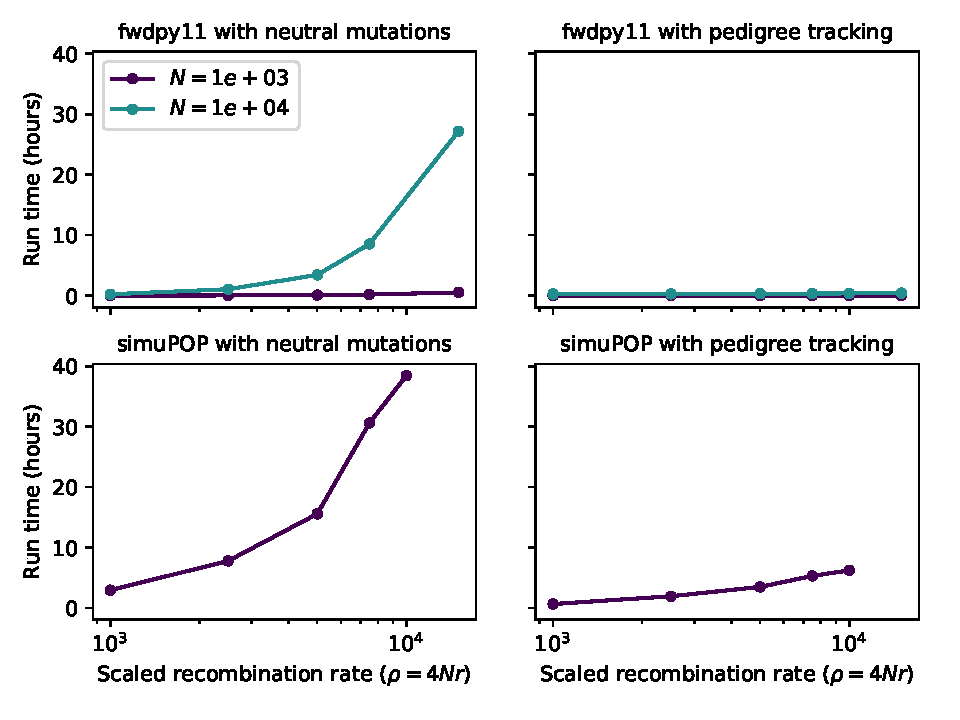
\includegraphics[]{sims/rawspeed_nosel}
    \caption{\label{sfig:rawspeed_nosel}Total run time for a single simulation replicate as a function of region
        length, measured as the scaled recombination parameter $\rho = 4Nr$.  The simulations here involve no natural
    selection.}
\end{figure}

\begin{figure}
    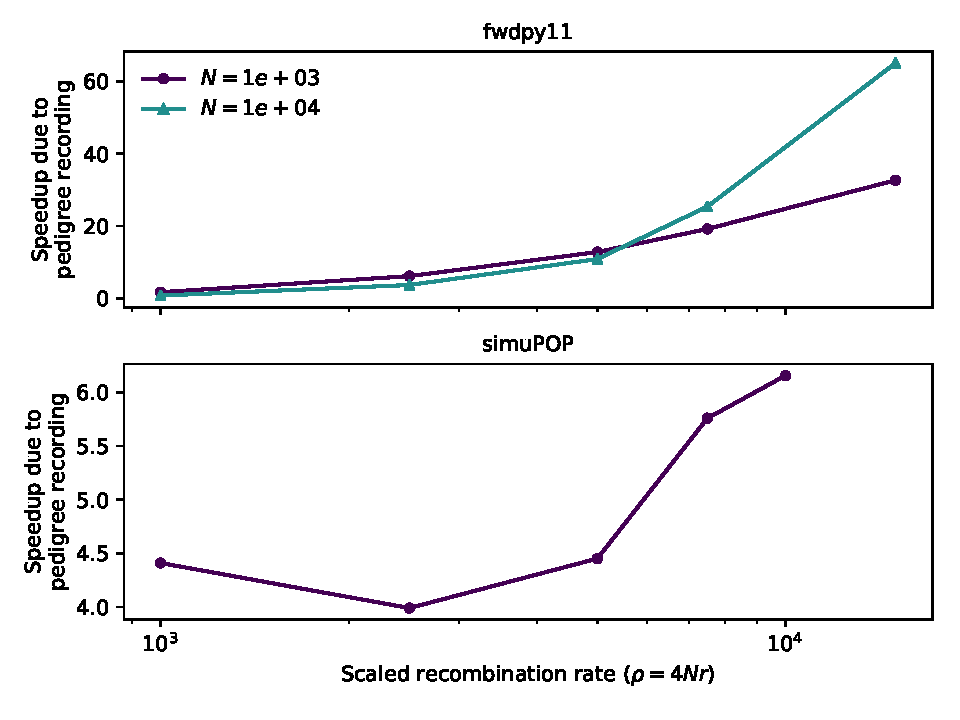
\includegraphics[]{sims/speedup_nosel}
    \caption{\label{sfig:speedup_nosel}Relative performance improvement due to pedigree tracking for simulations without
    selection.  Data points are taken from Figure~\ref{sfig:rawspeed_nosel} and show the ratio of run times tracking
neutral variation over the run times tracking the pedigree.}
\end{figure}

\end{document}
